\documentclass[spanish, fleqn]{article}
\usepackage[english]{babel}
\usepackage[utf8]{inputenc}
\usepackage{amsmath}
\usepackage{amsfonts}
\usepackage{wasysym}
\usepackage{mathrsfs}
\usepackage[colorlinks, urlcolor=blue]{hyperref}
\usepackage{fourier}
\usepackage{graphicx}
\usepackage[top = 2.5cm, bottom = 2cm, left = 2cm, right = 2cm]{geometry}
\usepackage{tikz}
\usepackage{tikz-qtree}
\usetikzlibrary{automata, positioning}

\title{
	Introducción a la Informática Teórica \\
	Tarea 3 \\
	``¡Opa Chomsky Style!''
	}
\author{
	Hernán Vargas Leighton \\
	201073009-3
	}

\date{16 de mayo 2014}

\begin{document}
	\maketitle
	\thispagestyle{empty}
	\section*{Respuestas}
%		Recuerde justificar todos sus resultados. Si no pudo resolver algo 
%		explique por qué, indicando los supuestos necesarios. Esta tarea le
%		ayudará, pero no reemplaza su estudio personal.
	\subsection*{Gramáticas}
		\begin{enumerate}
			\item 
%				En la tarea anterior usted debería haber comprobado que el 
%				lenguaje de los palíndromos no era regular.Ahora que cuenta con
%				las herramientas para crear palíndromos, construya la gramática
%				libre de contexto que genera palíndromos bajo el alfabeto
%				\(\Sigma = \{a, b\}\).
				Digamos $G = (\Sigma, N, P, S)$ la gramática de libre 
				contexto con:
				\begin{equation*}
					\Sigma = \{ a, b\} \\
					N = \{S, A, B\} \\
					P =
					\begin{Bmatrix}
						S \rightarrow A|B \\
						A \rightarrow aSa|aa|a \\
						B \rightarrow bSb|bb|b
					\end{Bmatrix}
				\end{equation*}
				Con $S$ símbolo de partida.\\
				Luego $G$ genera los palíndromos.

			\item
%				Un problema clásico cuando lidiamos con expresiones es la 
%				cantidad y tipo de paréntesis involucrados. Considere los
%				paréntesis llave \textbf{\{\}}, corchete \textbf{[]} y redondos
%				\textbf{()}. Encuentre la gramática que genera todas las
%				cadenas de paréntesis llave, corchete y redondos de forma
%				equilibrada. Note que no se deben generar pares de corchetes
%				que no sean del mismo tipo.
				Suponiendo $w$ cualquier expresión que puede ser encerrada por
				los paréntesis, además digamos que el string vacío $\epsilon$
				es un string con paréntesis equilibrados, tenemos que
				$G = (\Sigma, N, P, S)$ con:
				\begin{equation*}
					\Sigma = \Big \{(, ), \{, \}, [, ], w \Big \} \\
					N = \{S, A, B, C\} \\
					P =
					\begin{Bmatrix}
						S \rightarrow A|B|C|SS|w|\epsilon \\
						A \rightarrow (S) \\
						B \rightarrow [S] \\
						C \rightarrow \{S\}
					\end{Bmatrix}
				\end{equation*}
				Será la gramática que acepta cualquier expresión con paréntesis
				equilibrados.\\
				NOTA: $w$ puede ser reemplazado por cualquier alfabeto, por
				ejemplo, si decimos $w = x|y|z$ simplemente reemplazamos $w$ en
				$\Sigma$ y en $S$ y generamos strings con paréntesis
				equilibrados de la forma: $((x)y[{z}(x)]),\dots$

			\item 
%				La jerarquía de Chomsky consta de cuatro niveles. Explique
%				cuáles son, el tipo de gramáticas y de autómatas que
%				corresponden a cada nivel como se vio en clases.
				Los cuatro niveles de la jerarquía de Chomsky son:
				\begin{itemize}
					\item
						\textbf{Tipo 0:}
						\begin{itemize}
							\item 
								Lenguaje recursivamente enumerable.
							\item
								Gramática sin restricciones.
							\item
								Autómata: Máquina de Turing.
						\end{itemize}
					\item
						\textbf{Tipo 1:}
						\begin{itemize}
							\item
								Lenguaje sensible al contexto.
							\item
								Gramática: $\alpha \rightarrow \beta$ tal que
								$|\alpha| \leq |\beta|$
							\item
								Autómata: Linealmente acotado.
						\end{itemize}
					\item
						\textbf{Tipo 2:}
						\begin{itemize}
							\item
								Lenguaje de contexto libre.
							\item
								Gramática: Tipo 1 y al lado izquierdo solo un
								no terminal: $A \rightarrow B$ con $A \in N,
								B \in (N \cup \Sigma)^{*}$
							\item
								Autómata con pila (PDA)
						\end{itemize}
					\item
						\textbf{Tipo 3:}
						\begin{itemize}
							\item
								Lenguaje Regular.
							\item
								Gramática: Tipo 2 y al lado derecho a lo más un
							 	no terminal $A \rightarrow \alpha, 
								A \rightarrow \alpha B$ con $A,B \in N,
								\alpha \in \Sigma^{*}$
							\item
								Autómata finito. 
						\end{itemize}
				\end{itemize}

			\item
%				Para las siguientes preguntas utilice la misma gramática:
				Gramática para las operaciones aritméticas:
				\begin{itemize}
					\item
%						Construya una gramática cuyos strings representen 
%						operaciones aritméticas de la forma:
%						\((a+b)c-a\cdot b \dots \) con todas las operaciones
%						aritméticas conocidas. (\emph{ojo con las expresiones
%						inválidas}).
						Digamos $G=\{\Sigma, N, P, S\}$ con:
						\begin{equation*}
							\Sigma = \{(, ), +, -, \cdot, a, b\} \\
							N = \{S\} \\
							P = \Big \{ S \rightarrow 
								SS|(S)|S\cdot S|S+S|S-S|a|b \Big \}
						\end{equation*}
						Con $S$ símbolo de partida. $G$ representará las 
						operaciones aritméticas.

					\item
%						¿Usted cambiaría el alfabeto de terminales usado
%						anteriormente por \(\Sigma = \{x,y, z \}\)? Justifique.
						Se puede, nos basta con cambiar el alfabeto $\Sigma$
						para reemplazar $a,b$ por $x,y,z$ y hacer lo mismo en
						$G$:\\
						Ahora tenemos $G=\{\Sigma, N, P, S\}$ con:
						\begin{equation*}
							\Sigma = \{(, ), +, -, \cdot, x, y, z\} \\
							N = \{S\} \\
							P = \Big \{ S \rightarrow SS|(S)|S\cdot
								S|S+S|S-S|x|y|z \Big \}
						\end{equation*}
						NOTA: Se considera que el cambio en el alfabeto no
						afecta a los caracteres propios de una operación
						aritmética ($(,),+,-,\cdot$).

					\item
%						Dibuje el árbol de derivación para el string:
%						\begin{equation*}
%							(z -(x+y)(x-y))+zx-(x+y)\cdot z
%						\end{equation*}
						El árbol de derivación para $(z -(x+y)(x-y))+zx-(x+y)
						\cdot z$ será: \\

						\Tree [.S 
							[.S [.$($ ]
								[.S [.S z ]
									[.- ]
									[.S [.S [.$($ ]
											[.S [.S x ]
												[.+ ]
												[.S y ]
											]
											[.$)$ ]
										]
										[.S [.$($ ]
											[.S [.S x ]
												[.- ]
												[.S y ]
											]
											[.$)$ ]]
									]
								]
								[.$)$ ]
							]
							[.+ ]
							[.S [.S [.S z ]
									[.S x ]
								]
								[.- ]
								[.S [.S [.$($ ]
										[.S [.S x ]
											[.+ ]
											[.S y ]
										]
										[.$)$ ]
									]
									[.$\cdot$ ]
									[.S z ]
								]
							]
						]

					\item 
%						¿Es ambigua esta gramática? Demuestre su respuesta.
						La gramática es ambigua ya que existe más de una forma
						de hacer la derivación de extrema izquierda:
						\newcommand{\ra}{\rightarrow}
						\begin{gather}
							S \ra S+S \ra (S)+S \ra (S-S)+S\dots \\
							S \ra S-S \ra S+S-S \ra (S)+S-S \ra (S-S)+S-S \dots
						\end{gather}
						%TODO mejorar la referencia.
						(1) y (2) son diferentes formas de derivación de 
						extrema izquierda que nos llevan al mismo resultado
						(el árbol). \\
						Es más evidente (y menos costoso de escribir) para un
						string $x + y - z$, tenemos:
						\begin{gather*}
							S \ra S+S \ra x+S \ra x+S-S \ra x+y-S \ra x+y-z \\
							S \ra S-S \ra S+S-S \ra x+S-S \ra x+y-S \ra x+y-z
						\end{gather*}
						\\
					
					\item 
%						¿Su gramática está en CNF? Explique por que, y si no lo
%						es transfórmela.
						La gramática cumple con no tener $\epsilon$ ni 
						producciones unitarias ni producciones que no
						participen en la derivación del lenguaje 
						$\mathcal{L}(G)$, por lo tanto nos basta con escribirla
						de la forma $A\ra \alpha$, $A \ra BC$, entonces:
						\begin{gather*}
							S \ra x|y|z \\ A \ra ( \\ B \ra ) \\ C \ra + \\
							D \ra - \\ E \ra \cdot \\
							F \ra AS \\ G \ra SC \\ H \ra SD \\ I \ra SE \\
							S \ra SS|FB|GS|HS|IS
						\end{gather*}
						Será la gramática en forma normal de Chomsky.
				\end{itemize}
		\end{enumerate}

	\subsection*{PDA}
		\begin{enumerate}
			\item
%				Sea \(\Sigma = \{a,b\}\), construya el PDA que acepte el
%				lenguaje \(\mathscr{L} = \{w : w \in \Sigma^* \text{ y }w
%				\text{ tiene el doble de }a's\text{ que }b's\}\)
				El PDA que acepta $\mathscr{L} = w \in \Sigma$ tal que el string
				$w$ tiene el doble de $a's$ que $b's$ es $M =(Q,\Sigma,\Gamma,
				\delta, q_{0}, z_{0}, F)$ con:
				\begin{gather*}
					Q = \{q_0, q_1, q_2\} \\
					\Sigma = \{a,b\} \\
					\Gamma = \{Z,A,B\} \\
					\delta = \text{Función de transición} \\
					q_0 = q_0 \\
					F = \{q_2\}
				\end{gather*}
				Luego:
				\begin{center}
				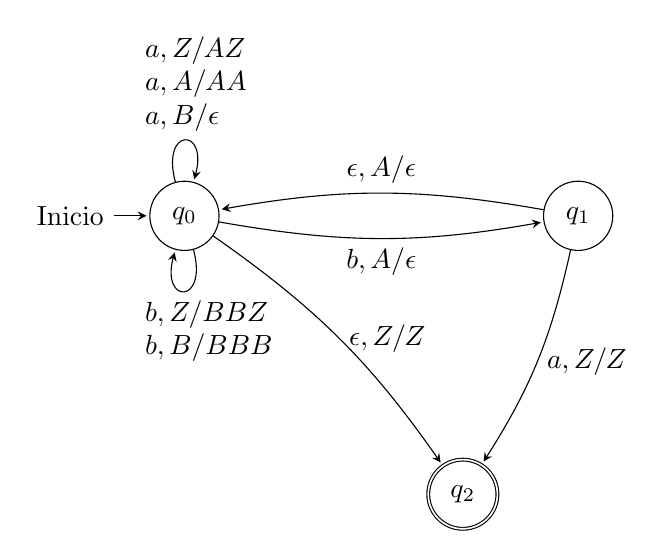
\begin{tikzpicture}[shorten >=1pt, node distance=5cm,
						on grid, >=stealth,	initial text=Inicio, bend angle=10]
				%%%%	NODOS	%%%%
					\node[state, initial]		(a)					{$q_0$};
					\node[state]				(b)[right=of a]		{$q_1$};
					\node[state, accepting]		(c)[below right=of a] {$q_2$};
				%%%%	CONEXIONES	  %%%%
					\path[->]
						(a)	edge[loop below] node[text width=1cm] 
							{$b, Z/BBZ$ $b, B/BBB$} ()
						(a)	edge[loop above] node[text width=1cm] 
							{$a, Z/AZ$ $a, A/AA$ $a, B/\epsilon$} ()
						(a)	edge[bend left] node[right] {$\epsilon , Z/Z$} (c)
						(b)	edge[bend left] node[right] {$a , Z/Z$} (c)
						(a)	edge[bend right] node[below] {$b, A/\epsilon$} (b)
						(b)	edge[bend right] node[above] {$\epsilon,
															A/\epsilon$} (a);
				\end{tikzpicture}
				\end{center}

			\item
%				Sea \(\Sigma = \{a,b\}\), construya el PDA que acepte el
%				lenguaje de todas las cadenas de \(a\)'s seguidas de \(b\)'s
%				seguidas de \(c\)'s tal que \(|a| + |c| = |b|\).
				Digamos $\mathscr{L}(M) = \{a^{x}b^{y}c^{z}: |a|+|c|=|b|\}$.
				Creamos el PDA $M = (Q, \Sigma, \Gamma, \delta, q_0, z_0, F)$
				tal que:
				\begin{gather*}
					Q = \{q_0, q_1, q_2, q_3\} \\
					\Sigma = \{a, b\} \\
					\Gamma = \{Z, A, B\} \\
					\delta = \text{Función de transición} \\
					q_0 = q_0 \\
					z_0 = Z \\
					F = \{ q_4 \}
				\end{gather*}
				Entonces:
				\begin{center}
				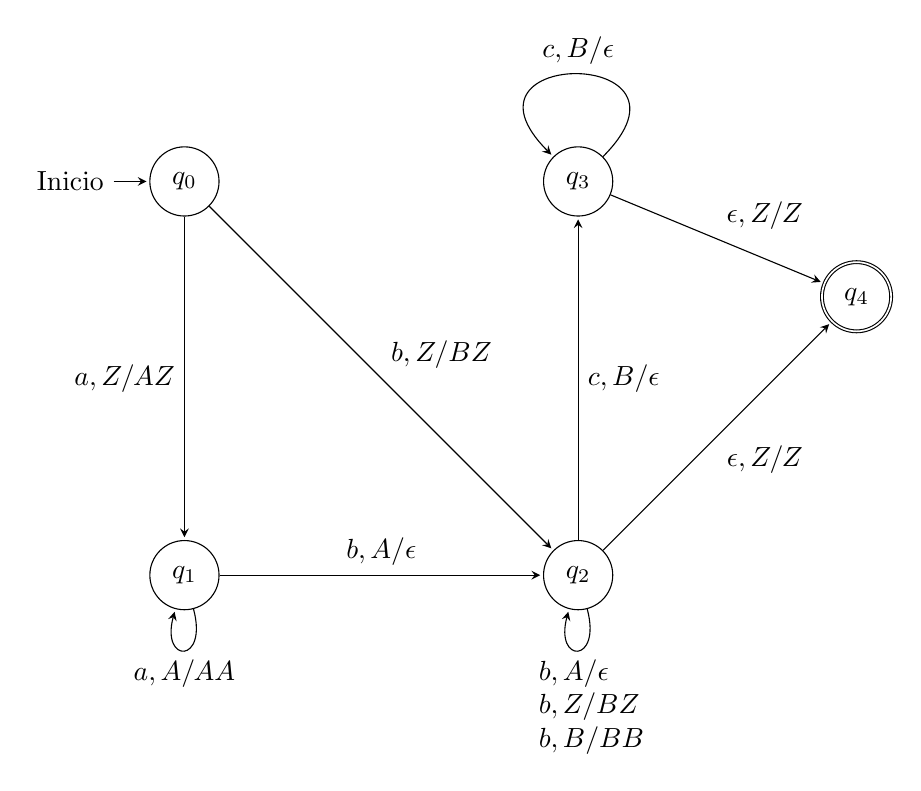
\begin{tikzpicture}[shorten >=1pt, node distance=5cm,
						on grid, >=stealth,	initial text=Inicio]
				%%%%	NODOS	%%%%
					\node[state, initial]		(a)					{$q_0$};
					\node[state]				(b)[below=of a]		{$q_1$};
					\node[state]				(c)[right=of b]		{$q_2$};
					\node[state]				(d)[right=of a]		{$q_3$};
					\node[state, accepting]		(e)[above right=of c] {$q_4$};
				%%%%	CONEXIONES	  %%%%
					\path[->]
						(a)	edge		node[left] {$a, Z/AZ$} (b)
						(a)	edge		node[above right] {$b, Z/BZ$} (c)
						(b)	edge[loop below]	node {$a, A/AA$} ()
						(b)	edge				node[above]{$b, A/\epsilon$}(c)
						(c)	edge[loop below]	node[text width=1cm]
							{$b, A/\epsilon$ $b, Z/BZ$ $b, B/BB $} ()
						(c)	edge		node[right] {$c, B/\epsilon$} (d)
						(c)	edge		node[below right] {$\epsilon, Z/Z$} (e)
						(d)	edge		node[above right] {$\epsilon, Z/Z$} (e)
						(d)	edge[loop]	node[above] {$c, B/\epsilon$} ();
				\end{tikzpicture}
				\end{center}
		\end{enumerate}

	\subsubsection*{Lema de Bombeo}
		\begin{enumerate}
			\item
%				El lema de bombeo es utilizado en general para demostrar cuando
%				un lenguaje no es regular (en su versión más simple).
%				Una forma de verlo es como un \emph{juego entre adversarios}.
%				Analizando esto, ¿Cuál cree que es un error frecuente al
%				momento de utilizar esta herramienta y que lo podría llevar a
%				obtener resultados erróneos?
				Creo que cuando queremos demostrar con el lema del bombeo que
				un lenguaje no es regular el error más frecuente tiene
				relación con elegir un string no adecuado o hacer mal la
				división $\alpha\beta\gamma$ y no poder demostrar para toda
				división que el lema no se cumple.\\
				En general estos errores están relacionados con hacer mal la
				negación del lema y, debido a ello, no poder probar la
				contradicción.

			\item
%				¿Es regular el lenguaje \(\mathscr{L}\)? Donde \(\mathscr{L}\)
%				es el lenguaje que posee un conjunto de cadenas de la forma
%				\(0^i 1^j\) tal que \( \gcd (i,j) = 1\).
				Supongamos el lenguaje $\mathscr{L} = \{0^i1^j: \gcd(i,j)=1\}$
				regular, entonces cumple con el lema del bombeo:
				\begin{itemize}
					\item
						Digamos $N \in \mathbb{N}_{0}$ constante del lema.
					\item 
						Digamos $w = 0^{i}1^{j} \in \mathscr{L}$ con $0< i< j$,
						además cumple con $|w| = i+j \geq N$ y $\gcd(i,j) = 1$.
					\item
						Digamos $\alpha = 0^{p} \land \beta = 0^{i-p} \land
						\gamma = 1^{j}$ será toda partición que cumple con
						$|\alpha\beta| = p + i - p = i \leq N \land |\beta| 
						\geq 1$

					\item
						Al bombear vemos que tenemos una cantidad de ceros
						igual a $p + k(i-p)$, por lo que con $k = 
						\frac{j-p}{i-p}$ tendríamos $j$ ceros y, por lo tanto,
						la misma cantidad de ceros que unos, así $\gcd(j,j) = 
						j \neq 1$

				\end{itemize}

		\end{enumerate}

	\subsection*{Autómatas y expresiones regulares}
		\begin{enumerate}
			\item
%				Determine si \(\mathscr{L} = \{a^nb^n: n = 2\}\) es regular.
				El lenguaje $\mathscr{L} = \{a^nb^n: n = 2\}$ es regular ya que
				$n$ es constante y igual a $2$ por lo tanto el lenguaje no es
				infinito y puede ser escrito como $\mathscr{L} = aabbb$.

			\item
%				Se definen para dos lenguajes regulares \(\mathscr{A}\) y
%				\(\mathscr{B}\) la operación \textsc{BMBMCHQBM}\((\mathscr{A},
%				\mathscr{B})\) que produce el lenguaje de los strings \(w\) así
%				$$\{w : w = a_1b_1a_2b_2 \cdots a_kb_k, a_i \in \mathscr{A}\,
%				\forall i \in [1,k], b_i \in \mathscr{B}\,
%				\forall i \in [1, k]\}$$
				Para los lenguajes regulares $\mathscr{A}$ y $\mathscr{B}$
				digamos $\Sigma_A, \Sigma_B$ los alfabetos respectivos, además
				digamos $\Sigma = \Sigma_A \cup \Sigma_B$ la unión de ambos
				alfabetos, buscamos mostrar que la operación 
				$\textsc{BMBMCHQBM}$ produce lenguajes regulares.

				\begin{itemize}
					\item
%						Muestre que la operación es regular a través de
%						autómatas.
						\textbf{Demostración usando un autómata:}
						Digamos $\alpha = a_i \forall i \in [1,k]$, $\beta = 
						b_i \forall i \in [1,k]$, tenemos:
						\begin{equation*}
							\Sigma = \{\alpha,\beta\} \\ Q = \{a,b\} \\
							q_0 = a \\ F = \{a\}
						\end{equation*}
						Entonces $M = (\Sigma, Q,\delta, q_o, F)$ será:
					\begin{center}
					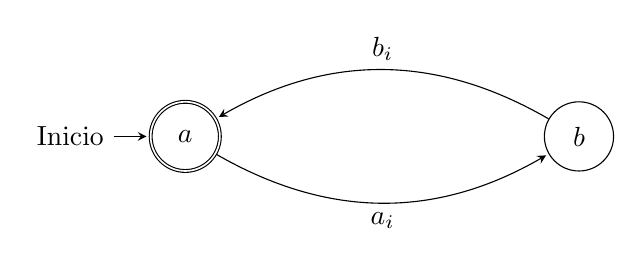
\begin{tikzpicture}[shorten >=1pt, node distance=5cm,
							on grid, >=stealth,	initial text=Inicio]
					%%%%	NODOS	%%%%
						\node[state, initial, accepting] (a) {$a$};
						\node[state] (b)[right=of a] {$b$};
					%%%%	CONEXIONES	  %%%%
						\path[->]
							(a)	edge[bend right]	node[below] {$a_i$} (b)
							(b)	edge[bend right]	node[above] {$b_i$} (a);
					\end{tikzpicture}
					\end{center}
					\item
%						Muestre que la operación es regular usando propiedades
%						de clausura.
						\textbf{Demostración usando propiedades de clausura:}
						Logramos la intercalación duplicando cada símbolo con
						todas las alternativas posibles, antes y después de él,
						según corresponda, así definimos las sustituciones:
						\begin{gather*}
							S_1(a) = {a} \cdot \Sigma \\
							S_2(a) = \Sigma \cdot {a} 
						\end{gather*}
						Con $\Sigma = \bigcup_{a\in\Sigma} \{A\}$ \\
						Luego debemos hacer la intercepción y el string
						resultante será justamente la intercalación pues es el
						único que se repite. Entonces:
						\begin{equation*}
							\textsc{BMBMCHQBM}(\mathscr{A}, \mathscr{B}) = 
							S_1(\mathscr{A}) \cap S_2(\mathscr{B})
						\end{equation*}

				\end{itemize}
		\end{enumerate}
 \vfill\hfill HV/\LaTeXe
\end{document}
